\section{Preliminares}\label{sec:preliminares}
  En esta sección, abordaremos la transformada y la serie de Fourier con el fin de desarrollar técnicas que nos ayuden a resolver distintos tipos de ecuaciones diferenciales parciales (EDPs). Primero, repasaremos conceptos básicos de espacios vectoriales que serán fundamentales para comprender la transformada de Fourier aplicada a diversas clases de funciones. A continuación, iniciaremos el análisis de la transformada de Fourier en el contexto de funciones periódicas. Vale la pena mencionar que seguimos de cerca los libros \cite{MR2597943} y \cite{MR3243734}, junto a las notas de clase, por que, realizar una lectura de estás será de buen provecho antes de empezar a leer el escrito.
  \subsection{Espacios Vectoriales}\label{subsec:espacios-vectoriales}
    En esta sección trataremos algunos conceptos que nos permitirán entender la profundidad y el trasfondo que hay detrás de la transformada de Fourier con el fin de que el lector y el escrito hablen un mismo idioma. No obstante, para mantener la concisión y evitar una extensión innecesaria del trabajo, algunos resultados se presentan sin la demostración detallada. Esta decisión se ha tomado para enfocar el contenido en los aspectos más relevantes del tema, sin sacrificar la claridad ni la comprensión general. Sin embargo, se asume que el lector tiene un conocimiento previo suficiente para aceptar estos resultados o se alienta a consultar fuentes adicionales para las pruebas completas de los mismos. Así, sin mucho más rodeo, comencemos.\\
    Sea $V$ un espacio vectorial real o complejo. La norma $\|\cdot\|:V\rightarrow [0,\infty)$ es una función que para todo $v_1,v_2\in V$ y $\alpha$ un escalar sobre $V$ cumple:
    \begin{enumerate}
      \item $\|v_1\|=0$ si y solo si $v_1=0$,
      \item $\|\alpha v_1\|=|\alpha|\|v_1\|$,
      \item \textit{desigualdad triangular}: $\|v_1+v_2\|\leq \|v_1\|+\|v_2\|$.
    \end{enumerate}
    Un espacio vectorial $V$ dotado con una norma $\|\cdot\|$ que satisface las condiciones anteriores, se llama un \textit{espacio vectorial normado}. Se suele denotar como $(V,\|\cdot\|)$.\\
    Recordamos que un \textit{espacio de Banach} es un espacio vectorial normado que es completo con respecto a la norma asignada.\\
    Un producto interno sobre un espacio vectorial complejo $V$ es una aplicación $(\cdot\mid\cdot):V\times V\rightarrow \mathbb{C}$ tal que para cualquier $vi,v2,v3 \in V$ y $\alpha,\beta \in \mathbb{C}$:
    \begin{enumerate}
      \item $(\alpha v_1+\beta v_2\mid v_3)=\alpha(v_1\mid v_3)+\beta(v_2\mid v_3)$,
      \item $(v_1\mid v_2)=\overline{(v_2\mid v_1)}$,
      \item $(v_1\mid v_1)\geq 0$, donde $(v_1\mid v_1)=0$ si y solo si $v_1=0$.
    \end{enumerate}
    Tenemos que el producto interno induce una norma en $V$ dada por $\|v_1\|=(v_1\mid v_1)^{\frac{1}{2}}$.\\
    En este caso se dice que la norma viene dada por un producto interno.\\
    Un \textit{espacio de Banach} cuya norma esta dada por un producto interno se llama un \textit{espacio de Hilbert}.\\
    Adicionalmente, dado un espacio vectorial $V$ real o complejo con producto interno $(\cdot\mid\cdot)$ (por ende, con norma $\|v\|=(v\mid v)^{\frac{1}{2}}$) vale la desigualdad de \textit{Cauchy-Bunyakovsky-Schwarz} (o \textit{Cauchy-Schwarz} por brevedad).
    $$|(v_1\mid v_2)|\leq \|v_1\|\|v_2\|,$$
    para $v_1,v_2\in V$.\\
    \begin{example}[Espacios Euclídeos]
      Sean $n\geq 1$ entero y $1\leq p \leq \infty$. $(\mathbb{R},\|\cdot\|_{p})$ es un espacio de Banach con cualquiera de las normas:
      \begin{align*}
        \|v\|=\left(\sum_{i=1}^{n}|v_i|^{p}\right)^{\frac{1}{p}},
      \end{align*}
      con $p<\infty$ y $v=(v_1,\cdots,v_n)\in\mathbb{R}^{n}$, cuando $p=\infty$, la norma es dada por:
      $$\|v\|_{\infty}=\sup_{1\leq i\leq n}|v_i|$$.\\
      Si $p=2$, entonces la norma es inducida por el producto interno $(v,w)=\sum_{i=1}^{n}v_iw_i$, para $v=(v_1,\cdots,v_n),w=(w_1,\cdots,w_n)\in\mathbb{R}^{n}$.\\
      Misma conclusión para $(\mathbb{C},\|\cdot\|_{p})$.
    \end{example}
    \begin{example}[Espacios $l^{p}$]
      Sea $1 < p < \infty$. Consideramos el siguiente conjunto de secuencias complejas.
      $$l^{p} =l^{p}(\mathbb{Z}):=\{\alpha = (\alpha_k)_{k\in\mathbb{Z}}: \alpha_k \in \mathbb{C} \text{ para todo }k, \sum_{k=-\infty}^{\infty}|\alpha_k|^{p} < \infty\}.$$
      Notamos que $l^{p}$ es un espacio vectorial complejo con la suma $(\alpha_k)_{k\in\mathbb{Z}} + (\beta_k)_{k\in\mathbb{Z}} =(\alpha_k +\beta_k)_{k\in\mathbb{Z}}$ y la multiplicación por escalar $\lambda\cdot(\alpha_k)_{k\in\mathbb{Z}} = (\lambda\alpha_k)_{k\in\mathbb{Z}}$, $\lambda \in \mathbb{C}$. Además, consideramos la norma:
      $$\|\alpha\|_{p}=\left(\sum_{k=-\infty}^{\infty}|\alpha_k|^{p}\right)^{\frac{1}{p}}.$$
      Se puede mostrar que $(l^{p}, \|\cdot\|)$ es un espacio de Banach. Cuando $p = \infty$, consideramos:
      $$l^{\infty} =l^{\infty}(\mathbb{Z}) := \{\alpha = (\alpha_k)_{k\in\mathbb{Z}} : \alpha_k \in \mathbb{C} \text{ para todo }k, \sup_{k\in\mathbb{Z}} |\alpha_k| < \infty\}$$
      y definimos la norma
      $$\|\alpha\|_{\infty} = \sup_{k\in\mathbb{Z}} |\alpha_k|.$$
      Tenemos que $(l^{\infty}, \|\cdot\|_{\infty})$ es un espacio de Banach.\\
      Cuando $p=2$, la norma es inducida por el producto interno:
      $$(\alpha\mid\beta)=\sum_{k=-\infty}^{\infty}\alpha_k\overline{\beta_k}$$
      donde $\alpha = (\alpha_k)_{k\in\mathbb{Z}}, \beta = (\beta_k)_{k\in\mathbb{Z}} \in l^{2}(Z)$.
    \end{example}
    \begin{example}[Norma $L^{p}$]
      para $1\leq p\leq \infty$ y $f\in C(B_r(a))$ definimos la norma:
      \begin{equation}
        \|f\|_p=\left(\int_{B_r(a)}|f(x)|^{p}dx\right)^{\frac{1}{p}}.\label{eq:n-Lp}
      \end{equation}
      Tenemos que $(C(B_r(a),\|\cdot\|_{p}))$ es un espacio vectorial normado que no es completo.\\
      Por otro lado, consideremos la norma:
      \begin{equation}
        \|f\|_{\infty}=\sup_{x\in B_{r}(a)}|f(x)|.\label{eq:n-infinito}  
      \end{equation}
      Se puede mostrar que $C(B_{r}(a),\|\cdot\|_{\infty})$ es un espacio de Banach.\\
      Cuando $p=2$, la norma es inducida por el producto interno:
      \begin{equation}
        (f\mid g)=\int_{B_{r}(a)}f(x)\overline{g(x)}dx.\label{eq:p.i-de-L2}
      \end{equation}
      La norma $\|\cdot\|_{p}$ se llama la norma $L^{p}$, $|\leq p\leq \infty$. La norma $L^{\infty}$ también se llama la norma del supremo o del $\sup$. 
    \end{example}
  \subsection{Funciones periódicas}\label{subsec:funciones-periodicas}
    Una función $f: \mathbb{R}^{n}\rightarrow \mathbb{C}$ se dice periódica de periodo $L\neq 0$, si
    $$f(x+L)=f(x),\hspace{1cm}\text{para todo $x\in\mathbb{R}^{n}$.}$$
    Algunas observaciones:
    \begin{itemize}
      \item Tenemos que para cualquier $k\in \mathbb{Z}$, $kL$ también es un periodo de $f$ en el sentido que $f(x + kL) = f(x)$, para cualquier $x \in \mathbb{R}^{n}$. En particular, $-L$ también es un periodo para la función $f$. Por esta razón se puede asumir que si $L=(L_1,\cdots,L_n)$, entonces $L_i>0$ para $i=1,\cdots,n$.
      \item Si $f$ es constante, entonces $f$ es periódica de cualquier periodo. Si $f$ es periódica no constante, existe un menor periodo $L$ con $L_i>0$ e $i=1,\cdots,n$, el cual se conoce como periodo fundamental.
    \end{itemize}
    \begin{example}
      Sea $k\in\mathbb{Z}^{+}$ y $L$ con $L_i>0$ para $i=1,\cdots,n$. Las funciones $f_k(x)=\sin\left( \frac{2k\pi}{L}x \right),g_k(x)=\cos\left( \frac{2k\pi}{L}x \right)$ son periódicas de periodo $L$, pero su periodo fundamental es $\frac{L}{k}$.  
    \end{example}
    Dado $L$ con $L_i>0$ para cada $i=1,\cdots,n$, llamaremos $L$-rectángulo al rectángulo $L_R:=[-L_1,L_1]\times\cdots\times[-L_n,L_n]$. Así, dado $L$ con las mismas condiciones anteriores el conjunto $C_{per}(L_R)$ consiste de todas las funciones $f : \mathbb{R}^{n}\rightarrow\mathbb{C}$ continuas con periodo $2L$. Similarmente, dado $k \in \mathbb{Z}^{+}, C_{per}^{k}(L_R)$ consiste de todas las funciones $f :\mathbb{R}^{n}\rightarrow\mathbb{C}$ periódicas con periodo $2L$ de clase $C^{k}$.\\
    De manera equivalente, los espacios anteriores se pueden identificar como sigue:
    $$C_{per}(L_R):=\{f\in C(L_R):f(-L)=f(L)\}$$
    Cuando $k \in \mathbb{Z}^{+}$,
    $$C_{per}^{k}(L_R):=\{f\in C^{k}(L_R):\partial^{\beta}f(-L)=\partial^{\beta}f(L)\},$$
    para todo multi-índice $\beta$ con $0\leq |\beta| \leq k$.\\
    Diremos que $f \in C_{per}^{\infty}(L_R)$, si $f \in C_{per}^{k}(L_R)$ para cualquier $k \in \mathbb{Z}^{+}$. Por consistencia en la notación, definimos $C_{per}^{0}(L_R)=C_{per}(L_R)$.\\
    De la definición de los espacios $C_{per}^{k}$ notamos que:
    $$C_{per}(L_R)\supseteq C_{per}^{1}(L_R)\supseteq\cdots\supseteq C_{per}^{k}(L_R)$$
    El espacio $C_{per}^{k}(L_R)$ es un espacio vectorial que resulta ser de Banach con la norma:
    \begin{equation}
      \|f\|_{\infty,k}=\sum_{j}\|\partial^{j}f\|_{\infty},  
    \end{equation}
    donde $j$ es un multi-índice tal que $0\leq |j|\leq k$ y la norma $\|\cdot\|_{\infty}$ es dada por $\textcolor{red}{\ref{eq:n-infinito}}$, con $r=|L|$ y $a=0$. Para $1\leq p<\infty$, podemos asignar la norma en $L^{p}$ como en $\textcolor{red}{\ref{eq:n-Lp}}$ con $r=|L|$ y $a=0$ al espacio $C_{per}^{k}(L_R)$. Se sigue que $(C_{per}^{k}(L_R),\|\cdot\|_{p})$ es un espacio normado que no es completo con respecto a la norma $L^{p}$, $1\leq p<\infty$.
    \begin{example}
      Dado $c\in\mathbb{C}$ fijo, las funciones $f(x)=\sin(x)$, $g(x)=c$ pertenecen a $C_{per}^{k}(\pi_R)$, para cualquier $k = 0,1,2,\cdots$. Es decir, $f,g \in C_{per}^{\infty}(\pi_R)$. Por otro lado, vea la Figura 2 para un ejemplo de una función $h \in C_{per}(\pi_R)$ con $h'\notin C_{per}(\pi_R)$.
      \begin{figure}[h]
        \caption{}
        \centering
        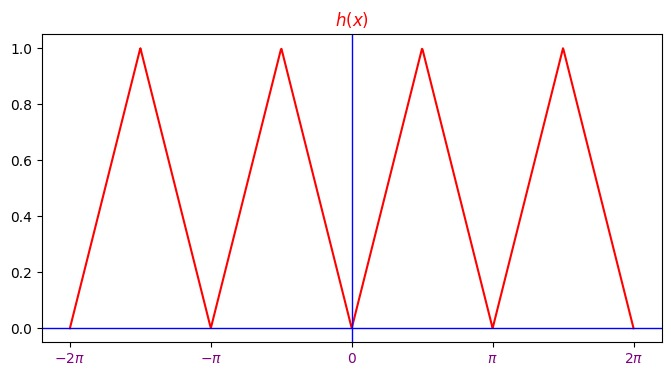
\includegraphics[width=0.8\textwidth]{h.jpeg}
      \end{figure}
      \begin{figure}[h]
        \caption{}
        \centering
        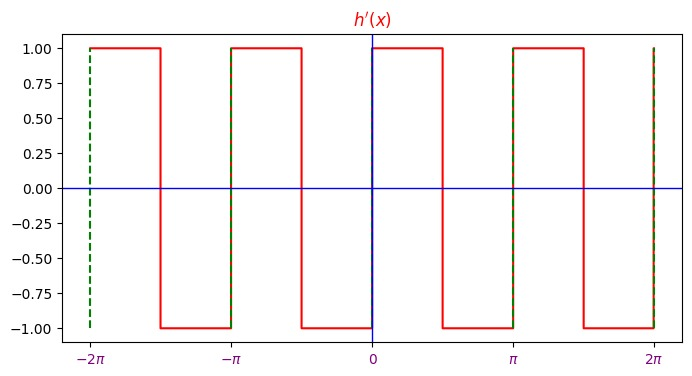
\includegraphics[width=0.8\textwidth]{h-prima.jpeg}
      \end{figure}        
    \end{example}
    \begin{note}\label{note:funcion-de-periodo-2pi}
      (i) Dado $L$ con $L_i>0$ para todo $i=1,\cdots,n$, si $f:\mathbb{R}^{n}\rightarrow\mathbb{C}$ es una función periódica de periodo $2L$, entonces\\
      \begin{align*}
        \tilde{f}(x):=f\left( \left( \frac{L_1}{\pi}x_1,\cdots,\frac{L_n}{\pi}x_n \right) \right)
      \end{align*}
      define una función periódica de periodo $2\pi$. En particular, obtenemos que los espacios $C_{per}^{k}(L_R)$ y $C_{per}^{k}(\pi_r)$ son isomorfos como espacios vectoriales. De igual manera, la teoría de la transformada de Fourier se puede reescalar para pasar de la bola $L_R$ a $\pi_R$. Por estas razones y sin pérdida de generalidad, en lo que sigue trabajaremos con funciones periódicas de periodo $2\pi$.\\
      (ii) Otra notación frecuente para funciones periódicas y transformada de Fourier es considerar funciones sobre el toro $\mathbb{T}^{n}$. El toro $\mathbb{T}$ es el intervalo $[0,2\pi]$ donde los lados opuestos se identifican. De manera más precisa, el toro es el conjunto de clases de equivalencia en $\mathbb{R}$ dada por la relación $x\sim y$ si y solo si $x-y \in 2\pi\mathbb{Z}$, es decir $\mathbb{T}=\mathbb{R}/2\pi\mathbb{Z}$. Geométricamente el toro es un circulo que se obtiene de doblar el segmento $[0,2\pi]$ uniendo los extremos del intervalo, por lo que $\mathbb{T}$ se puede ver como el subconjunto de $\mathbb{C}$ dado por:
      $$\{e^{ix}:x\in[0,2\pi]\}$$
      Por tanto, funciones $f: \mathbb{T}\rightarrow\mathbb{C}$ se pueden identificar como funciones periódicas $f:\mathbb{R}\rightarrow\mathbb{C}$ con periodo $2\pi$. De esta manera, $C_{per}^{k}(\pi_R)$, es isomorfo a $C^{k}(\mathbb{T}^n)$ por lo que en muchas aplicaciones se trabajan estos espacios como el mismo conjunto. No usaremos esta notación para funciones periódicas, no obstante, vea \cite{MR3243734} para un tratamiento de funciones sobre $\mathbb{T}^n$.
    \end{note}
  \subsection{Transformada de Fourier}
    Motivado por el problema mixto para la ecuación del calor en las notas de clase y su solución por el método de separación de variables, buscamos dar una teoría que justifique expansiones en series trigonométricas de la forma:
    $$f(x)=\sum_{k\in\mathbb{Z}^{+^n}\setminus (0,1)^{n}}b_k\sin\left( \pi k\cdot \frac{1}{L}\cdot x \right),$$
    donde:
    $$b_k=\frac{2}{L}\int_{L_R}f(x)\sin\left( \pi k\cdot \frac{1}{L}\cdot x \right)dx.$$
    Para esto y teniendo en cuenta la nota $\textcolor{red}{\ref{note:funcion-de-periodo-2pi}}$, primero trabajaremos con funciones $f\in C_{per}(\pi_R)$, es decir, funciones periódicas de periodo $2\pi$.\\
    Dada $f \in C_{per}(\pi_R)$ buscamos representar esta función en términos de una serie trigonométrica de la forma:
    \begin{equation}
      \frac{a_0}{2}+\sum_{k\in\mathbb{Z}^{+^n}}(a_k\cos(k\cdot x)+b_k\sin(k\cdot x)).\label{eq:serie-de-fourier}  
    \end{equation}
    Usando la exponencial compleja tenemos:
    \begin{align*}
      \cos(k\cdot x)=\frac{e^{ik\cdot x}+e^{-ik\cdot x}}{2}\hspace{0.5cm},\hspace{0.5cm}\sin(k\cdot x)=\frac{e^{ik\cdot x}-e^{-ik\cdot x}}{2i}  
    \end{align*}
    luego se cumple que:
    \begin{align*}
        \frac{a_0}{2}+\sum_{k\in\mathbb{Z}^{+^n}}(a_k\cos(k\cdot x)+b_k\sin(k\cdot x))&=\frac{a_0}{2}+\sum_{k\in\mathbb{Z}^{+^n}}a_k(\frac{e^{ik\cdot x}+e^{-ik\cdot x}}{2})+b_k(\frac{e^{ik\cdot x}-e^{-ik\cdot x}}{2i}),\\
        &=\frac{a_0}{2}\sum_{k\in\mathbb{Z}^{+^n}}\left(\frac{a_k-ib_k}{2}\right)e^{ik\cdot x}+\left(\frac{a_k+ib_k}{2}\right)e^{-ik\cdot x},\\
        &=\frac{a_0}{2}\sum_{k\in \mathbb{Z}^{+^n}}c_ke^{ik\cdot x}+c_{-k}e^{-ik\cdot x},\\
        &=\sum_{k\in\mathbb{Z}^n}c_ke^{ik\cdot x}.
    \end{align*}
    por lo que se concluye que $\textcolor{red}{\ref{eq:serie-de-fourier}}$ es equivalente a:
    $$\sum_{k\in\mathbb{Z}^{n}}c_ke^{ik\cdot x},$$
    donde $c_0=\frac{a_0}{2},c_k=\frac{a_k-ib_k}{2}$ y $c_{-k}=\frac{a_k+ib_k}{2}$, para $k\in\mathbb{Z}^{+^{n}}$. De esta manera, para representar a $f$ como:
    \begin{equation}
      f(x)=\sum_{k\in\mathbb{Z}^{n}}c_ke^{ik\cdot x}.\label{eq:serie-de-f}
    \end{equation}
    Antes de continuar introduzcamos algo de notación. Dado $k\in\mathbb{Z}^n$, definimos:
    \begin{equation}
        \Phi_{k}(x)=e^{ik\cdot x}
    \end{equation}
    Notamos que $\Phi_k\in C^{\infty}_{per}(\pi_R)$, además si $(\cdot|\cdot)$ denota el producto interno en $L^2$ dado por $\textcolor{red}{\ref{eq:p.i-de-L2}}$, por lo que tenemos que:
    \begin{align}
      \left( \Phi_k \mid \Phi_j \right) &= \int_{\pi_R} \Phi_k(x) \overline{\Phi_j(x)} dx\notag\\ 
      &= \int_{\pi_R} e^{ik\cdot x} e^{-ij\cdot x}dx\notag{}\\
      &=\int_{\pi_R}e^{i(k-j)\cdot x}dx= 
      \begin{cases} 
        0, & \text{si } j \neq k, \\\label{eq:ortogonalidad-de-phi} 
        (2\pi)^n, & \text{si } j = k.
      \end{cases}
    \end{align}
    El caso $0$ cuando $j\neq k$ se tiene ya que suponiendo $y=j-k$:
    \begin{align*}
      \int_{\pi_R}e^{iy\cdot x}dx&=\int_{\pi_R}e^{i\sum_{j=1}^{n}y_jx_j}dx,\\
      &=\prod_{j=1}^{n}\int_{-\pi}^{\pi}e^{iy_jx_j}dx_j,\\
      &=\prod_{j=1}^{n}\left(-\frac{ie^{iy_j\pi}}{y_j}+\frac{ie^{-iy_j\pi}}{y_j}\right),\\
      &=\prod_{j=1}^{n}\left( -\frac{i(-1)^{y_j}}{y_j}+\frac{i(-1)^{-y_j}}{y_j} \right),\\
      &=\prod_{j=1}^{n}(0),\\
      &=0,
    \end{align*}
    ya que $(-1)^{-y_j}=(-1)^{y_j}$.\\
    Suponiendo que la identidad $\textcolor{red}{\ref{eq:serie-de-f}}$ se tiene y la serie converge uniformemente se puede concluir que:
    \begin{align*}
      (f\mid \Phi_k)&=\sum_{z\in\mathbb{Z}^{n}}c_z(\Phi_k\mid \Phi_z),\\
      &=(2\pi)^{n}c_k.
    \end{align*}
    De lo que se sigue que:
    \begin{align*}
      c_k&=\frac{1}{(2\pi)^{n}}(f\mid \Phi_k),\\
      &=\frac{1}{(2\pi)^{n}}\int_{\pi_R}f(x)e^{-ik\cdot x}dx.
    \end{align*}
    \begin{definition}
      Dada $f\in C_{per}(\pi_R)$ la secuencia de números complejos $\{\hat{f}(k)\}_{k\in\mathbb{Z}^{n}}$  se llama la transformada de Fourier de $f$ y está definida como:
      \begin{equation}
        \hat{f}(k)=\frac{1}{(2\pi)^n}\int_{\pi_R}f(x)e^{-ik\cdot x}dx\label{eq:transformada-de-f-en-k}  
      \end{equation}
      Al número complejo $\hat{f}(k)$ se le llama el coeficiente de Fourier.\\
      \textit{La serie (puede ser no convergente)}
      \begin{equation}
        \sum_{k\in\mathbb{Z}^{n}}\hat{f}(k)e^{ik\cdot x},\label{eq:serie-transformada-de-f} 
      \end{equation}
      se llama la serie de Fourier de $f$.
    \end{definition}
    Notemos que si $f\in C_{per}(\pi_R)$, entonces:
    \begin{align*}
      |\hat{f}(k)|&\leq\frac{1}{(2\pi)^{n}}\int_{\pi_R}|f(x)e^{-ik\cdot x}|dx,\\
      &\leq\frac{1}{(2\pi)^{n}}\int_{\pi_R}|f(x)|dx,\\
      &\leq \frac{1}{(2\pi)^{n}}\|f\|_{L^1},\\
      &\leq \|f\|_{\infty}.
    \end{align*}
    Por lo que recordando la norma del espacio de secuencias $l^{\infty}(\mathbb{Z}^{n})$, se tiene que:
    \begin{equation}
      \|\{\hat{f}(k)\}_{k\in\mathbb{Z}^{n}}\|_{\infty}=\sup_{k\in\mathbb{Z}^{n}}|\hat{f}(k)|\leq \|f\|_{\infty}.\label{eq:cota-transformada-l-infinito}
    \end{equation}
    De esta manera podemos concluir.
    \begin{proposition}
      La aplicación
      $$\wedge:(C_{per}(\pi_R),\|\cdot\|_{\infty})\rightarrow l^{\infty}(\mathbb{Z}^{n}),\text{ dada por $f:\longmapsto \hat{f}:=\{\hat{f}(k)\}_{k\in\mathbb{Z}^{n}}$ }$$
      es lineal y continua.
    \end{proposition}
    Note que esto es fácil de demostrar, ya que la linealidad se es heredada de la linealidad de la integral y la continuidad se tiene gracias a que si $f\in C_{per}(\pi_R)$, entonces $\|f\|_{\infty}<\infty$, luego por la desigualdad $\textcolor{red}{\ref{eq:cota-transformada-l-infinito}}$ tenemos asegurado un argumento por límite (esto se deja como ejercicio al lector).\\
    Una propiedad muy útil de la transformada de Fourier es la relación entre diferenciabilidad y decaimiento. Más precisamente estudiemos la siguiente proposición.
    \begin{proposition}
      Sea $\beta$ un multi-índice de orden $l$ y $f\in C^{l}_{per}(\pi_R)$, entonces
      \begin{equation}
        \hat{\partial^{\beta}f}(k)=(i)^{|\beta|}(k)^{\beta}\hat{f}(k),\phantom{xxx}k\in\mathbb{Z}^{n}.\label{eq:transformada-de-la-derivada} 
      \end{equation}
    \end{proposition}
    \begin{proof}
      Si $\beta$ es un multi-índice de orden 1, entonces $\partial ^{\beta}$ no es más que una derivada parcial de orden 1, llamémosla $\partial x_{j}$ para $1 \leq j \leq n$. Teniendo en cuenta que $f$ es de clase $C^{1}$ y nuestro $\pi_R$ es compacto por ser producto de intervalos compactos, podemos aplicar el teorema de Fubini e integramos primero respecto a $x_{j}$, como sigue 
      \begin{align*}
        \hat{\partial x_{j}f} (k) &= \int_{\pi_R} \partial x_{j} f(x) \Phi _{k}(x) dx\\ 
        &= \int_{[-\pi,\pi]^{n-1}}\left( \int_{[-\pi,\pi]}\partial x_{j} f(x) e^{-ikx}dx_{j} \right)d\bar{x}
      \end{align*}
      Integramos por partes, y usamos la periodicidad del integrando para eliminar el término de frontera. Luego,
      \begin{align*}
        \hat{\partial x_{j}f} (k) &= \int_{[-\pi,\pi]^{n-1}}\left( ik_{j} \int_{[-\pi,\pi]} f(x) e^{-ikx}dx_{j} \right)d\bar{x}\\ 
        &= ik_{j} \int_{\pi_R} f(x)e^{-ikx}dx\\ 
        &= ik_{j} \widehat{f}(k).\\ 
        &= i^{|1|} \cdot 1 \cdot ... \cdot 1 \cdot k_{j} \cdot 1 \cdot ... \cdot 1 \cdot \widehat{f}(k)\\ 
        &= i^{|\beta|} (k_{1},...,k_{n})^{(0,...,0,1,0,...,0)} \widehat{f}(k) \hspace{1cm} \text{(1 en la j-ésima posición) }\\
        &= i^{|\beta|} k^{\beta} \widehat{f}(k)
      \end{align*}
      Ahora, supongamos que $f \in C^{l}(\pi_R)$ y $\hat{\partial^{\beta}f}(k) = i^{|\beta|}k^{\beta}\widehat{f}(k)$ para todo multi-índice $\alpha$ de orden $l$ para algún $ l\geq 1$. Ahora supongamos $f\in C^{l+1}(\pi_R)$ y $\beta$ multi-índice de orden $l+1$. Note que podemos interpretar a $\partial ^{\beta} f$ como $\partial x_{j} (\partial ^{\alpha}f)$ con $1\leq j \leq n$ y  $\alpha$ multi-índice de orden $l$. La regularidad de $f$ nos permite proceder justo como en la prueba anterior, cambiando a $f$ por $\partial^{\alpha}f$, de modo que
      \begin{align*}
        \hat{\partial ^{\beta}f}(k) &= \hat{\partial x_{j}(\partial^{\alpha}f)}(k)\\
        &= ik_{j} \widehat{\partial ^{\alpha}f}(k)\\ 
        &= ik_{j} \cdot i^{|\alpha|} k^{\alpha} \widehat{f}(k)\\
        &= i^{|\alpha|+1} k_{1}^{\alpha_{1}}...k_{j}^{\alpha_{j}+1}...k_{n}^{\alpha_{n}} \widehat{f}(k)\\ 
        &= i^{|\beta|} k^{\beta} \widehat{f}(k)
      \end{align*}  
    \end{proof}
    \begin{note}
      La identidad \textcolor{red}{\ref{eq:transformada-de-la-derivada}} nos muestra una de las propiedades claves en aplicaciones de la transformada de Fourier, pues este operador permite convertir problemas con derivadas en problemas algebraicos de multiplicación por polinomios.\\
      Esto presenta varias ventajas a la hora de buscar o simular soluciones, por ejemplo, en el desarrollo de métodos numéricos como los métodos espectrales.
    \end{note}
    Veamos algunas propiedades de convergencia de la serie de Fourier.
    \begin{theorem}\label{theorem:convergencia-c1}
      Sea $f\in C_{per}(\pi_R)$, entonces:
      \begin{enumerate}
        \item La serie $\sum_{k\in\mathbb{Z}^{n}}|\hat{f}(k)|^{2}$ converge absolutamente. Más aún, vale la desigualdad de Bessel.
          \begin{equation}
            \sum_{k\in\mathbb{Z}^{n}}|\hat{f}(k)|^2\leq \frac{1}{(2\pi)^2}\|f\|_{2}^{2} \label{eq:desigualdad-de-bessel}
          \end{equation}
        \item (Lema de Riemman-Lebesgue).\\
          \begin{align*}
            \lim_{|k| \rightarrow \infty}\hat{f}(k)=0.
          \end{align*}
        \item Sea $f\in C^{1}_{per}(\pi_R)$. Entonces la serie de Fourier de $f$, es decir, $\textcolor{red}{\ref{eq:serie-transformada-de-f}}$ converge absoluta y uniformemente a $f$, es decir,
          \begin{align*}
            f(x)&=\sum_{k\in\mathbb{Z}^{n}}\hat{f}(k)e^{ik\cdot x},
          \end{align*}
          para todo $x\in\pi_R$.
        \item Sea $f\in C^{m}_{per}(\pi_R)$ con $m>\frac{n}{2}$ entero, entonces vale la identidad de Parseval:
          \begin{equation}
            \|\hat{f}\|_{2}^{2}=\sum_{k\in\mathbb{Z}^{n}}|\hat{f}(k)|^2=\frac{1}{(2\pi)^{n}}\int_{\pi_R}|f(x)|^2dx=\frac{1}{(2\pi)^n}\|f\|_2^2\label{eq:identidad-de-parseval}  
          \end{equation}
          De manera equivalente, si $g\in C^{m}_{per}(\pi_R)$,
          \begin{equation}
            (\hat{f}|\hat{g})=\sum_{k\in\mathbb{Z}^{n}}\hat{f}(k)\overline{\hat{g}(k)}=\frac{1}{(2\pi)^n}\int_{\pi_R}f(x)\overline{g(x)}dx=\frac{1}{(2\pi)^n}(f|g).\label{eq:identidad-de-parseval-prod-int}
          \end{equation}
      \end{enumerate}
    \end{theorem}
    \begin{note}
      Existen resultados más generales con diferentes hipótesis sobre $f$ que garantizan que la serie de Fourier converge puntual a $f$.\\
      Sin embargo, para nuestros objetivos estudiaremos la convergencia uniforme de la serie de Fourier en el caso que $f \in C^{m}_{per}(\pi_R)$, es decir, la parte (3) del Teorema $\textcolor{red}{\ref{theorem:convergencia-c1}}$.
    \end{note}
    Veamos la demostración del teorema $\textcolor{red}{\ref{theorem:convergencia-c1}}$.
    \begin{proof}
    \begin{enumerate}
      \item Desigualdad de Bessel.\\
        Consideremos la norma $L^2$ como en \textcolor{red}{\ref{eq:n-Lp}} con producto interno $(\cdot|\cdot)$ dado por $\textcolor{red}{\ref{eq:p.i-de-L2}}$. Luego, para $N\geq 0$ entero tenemos:
        \begin{align*}
          0 & \leq ||f - \sum_{|k| \leq N} \widehat{f}(k) \Phi _{k} ||^{2}_{2}\\ 
          &= \left( f - \sum_{|k| \leq N} \widehat{f}(k) \Phi _{k} \left| f - \sum_{|k| \leq N} \widehat{f}(k) \Phi _{k} \right. \right)\\ 
          &= \left( f  \left| f - \sum_{|k| \leq N} \widehat{f}(k) \Phi _{k} \right. \right) - \left(\sum_{|k| \leq N} \widehat{f}(k) \Phi _{k} \left| f - \sum_{|k| \leq N} \widehat{f}(k) \Phi _{k} \right. \right)\\ 
          &= \left( f  \left| f \right. \right) - \sum_{|k| \leq N} \overline{\widehat{f}(k)} \left( f  \left| \Phi _{k} \right. \right) - \sum_{|k| \leq N} \widehat{f}(k) \left( \Phi _{k} \left| f \right. \right) + \left(\sum_{|k| \leq N} \widehat{f}(k) \Phi _{k} \left| \sum_{|\bar{k}| \leq N} \widehat{f}(\bar{k}) \Phi _{\bar{k}} \right. \right)\\
        \end{align*}
        Hagamos una pausa primero, para notar que el segundo y tercer sumando son exactamente el mismo término por la definición de la transformada de Fourier, y tras usar la sesquilinealidad del producto interno y la ortogonalidad de las $\Phi _{k}$ (\textcolor{red}{\ref{eq:ortogonalidad-de-phi}}) en el último término llegamos a la siguiente expresión.
        \begin{align*}
          0 & \leq ||f||^{2}_{2} - 2 (2\pi)^{n} \sum_{|k| \leq N }|\widehat{f}(k)|^{2} - (2\pi)^{n} \sum_{|k| \leq N}|\widehat{f}(k)|^{2}\\ 
          &= ||f||^{2}_{2} - (2 \pi)^{n} \sum_{|k|\leq N}|\widehat{f}(k)|^{2} 
        \end{align*}
        De donde concluimos $\displaystyle \sum_{|k|\leq N}|\widehat{f}(k)|^{2} \leq \dfrac{1}{(2\pi)^{n}}||f||^{2}_{2s}$ para cualquier entero $N \geq 0$, lo que nos permite concluir al tomar $N\rightarrow \infty$ que la inecuación $\textcolor{red}{\ref{eq:desigualdad-de-bessel}}$ es verdadera.
      \item (Lema de Riemman-Lebesgue).\\
        Este resultado se sigue de la demostración anterior (1), ya que para que la expresión $\sum_{k\in\mathbb{Z}^{n}}|\hat{f}(k)|^2$ sea convergente, la sucesión $\{|\hat{f}(k)|^2\}_{k\in\mathbb{Z}^{n}}$ tiene que ir a $0$ cuando $|k|\rightarrow \infty$.
      \item (Convergencia de la serie de Fourier a $f$).\\
        Antes de deducir la convergencia de la serie de Fourier a $f$, veamos primero que esta converge absoluta y uniformemente. Por el criterio \textit{M de Weierstrass}\footnote{El criterio \textit{M de Weierstrass} dice que si para una secuencia de funciones $\{f_{k}(x)\}$ sobre un conjunto $X$ existe una secuencia $\{M_k\}$ de números no negativos, tales que $|f_{k}(x)| < M_k$, para todo $x\in X$ y todo $k$, además, si $\sum M_k$, es finita, entonces $\sum f_k(x)$ converge absoluta y uniformemente.} es suficiente con mostrar que:
        \begin{align*}
          \sum_{k\in\mathbb{Z}^{n}}\hat{f}(k)e^{ik\cdot x}\leq \sum_{k\in\mathbb{Z}^{n}}|\hat{f}(k)|<\infty.
        \end{align*}
        Para ver esto, usando que $f\in C^{m}_{per}(\pi_R)$ tenemos que \textcolor{red}{\ref{eq:transformada-de-la-derivada}} vale para $\beta$ multi-índice de orden $m$, esto y la desigualdad de Cauchy-Schwarz en $\mathbb{C}^{2N}$ nos dicen:
        \begin{align}
          \sum_{k\in N_R}|\hat{f}(k)|&\leq |\hat{f}(0)|+\sum_{0<|k|\leq |N|}|\hat{f}(k)|\notag{}\\
          &\leq |\hat{f}(0)|+\sum_{0<|k|\leq |N|}\frac{|\hat{\partial^{\beta}f}(k)|}{|k^{\beta}|}\notag{}\\
          &\leq |\hat{f}(0)|+\left( \sum_{0<|k|\leq|N|}|\hat{\partial^{\beta}f}(k)|^{2} \right)^{\frac{1}{2}}\left( \sum_{0<|k|\leq |N|}\frac{1}{|k^{\beta}|^2}\right)^{\frac{1}{2}}\notag{}\\
          &\leq |\hat{f}(0)|+C\|\partial^{\beta}f\|_{2}^{2},\label{eq:2-17}
        \end{align}
        para alguna constante $C>0$ (la cual realmente depende de $\sum_{0<|k|\leq |N|}\frac{1}{|k^{\beta}|^2}$), donde en la última linea de la desigualdad usamos la desigualdad de Bessel $\textcolor{red}{\ref{eq:desigualdad-de-bessel}}$ con $\partial^{\beta}f$.\\
        Por otro lado, puesto que ya sabemos que la serie de Fourier converge uniformemente, solo nos resta ver que esta converge puntualmente a $f$. Para esto, primero necesitamos el siguiente resultado.
        \begin{proposition}\label{proposition:2.13}
          Suponga $g\in C^{m}_{per}(\pi_R)$, entonces
          \begin{align*}
            \sum_{k\in\mathbb{Z}^{n}}\hat{g}(k)=g(0).
          \end{align*}
        \end{proposition}
        \begin{proof}
          Se deja como ejercicio al lector.  
        \end{proof}
        Retornando a la convergencia puntual de la serie de Fourier a $f$, consideramos $x_0 \in \pi_R$ arbitrario pero fijo. Definimos la función:
        \begin{align*}
          g(x) = f(x + x_0), \quad x \in \pi_R.            
        \end{align*}
        Se sigue que $g \in C^{m}_{per}(\pi_R)$, $g(0) = f(x_0)$. Además, haciendo un cambio de variable se puede ver que:
        \begin{align*}
          \hat{g}(k) = \begin{cases} 
            \hat{f}(k)e^{ik\cdot x_0}, & \text{si } k \neq 0, \\
            f(0), & \text{si } k = 0.
            \end{cases}
        \end{align*}
        De esta manera, aplicando la Proposición \textcolor{red}{\ref{proposition:2.13}} llegamos a:
        \begin{align*}
          f(x_0)=g(0)=\sum_{k\in\mathbb{Z}^{n}}\hat{g}(k)=\sum_{k\in\mathbb{Z}^{n}}\hat{f}(k)e^{ik\cdot x_0},
        \end{align*}
        es decir, la serie de Fourier converge a la función $f$ en el punto $x_0$. Puesto que este punto es arbitrario y la sserie converge uniformemente, se completa la demostración de $(3)$.
      \item (Identidad de Parseval).\\
        Dada la convergencia uniforme de la serie de Fourier a la función dada en (3), la identidad de Parseval es una consecuencia de la propiedad que permite pasar el limite uniforme dentro y fuera de la integral sobre un compacto.
    \end{enumerate}
    \end{proof}
    \begin{note}
      Recordando el espacio $l^1(\mathbb{Z}^{n})$, notamos que si $f \in C^{m}_{per},(\pi_R)$ con $m>\frac{n}{2}$ entero y $\beta$ multi-índice de orden $m$ distinto del nulo, entonces por \textcolor{red}{\ref{eq:2-17}} tenemos que existe una constante $C > 0$ independiente de $f$ tal que:
      \begin{equation}
        \|\hat{f}\|_{l^1}\leq C(\|f\|_{\infty}+\|\partial^{\beta}f\|_{\infty})  
      \end{equation}
      En particular, la aplicación:
      $$\wedge:C^{1}_{per}(\pi_R)\rightarrow l^1(\mathbb{Z}^{n}),\phantom{xxx}\text{ dada por }f\longmapsto \hat{f}:=\{\hat{f}(k)\}_{k\in\mathbb{Z}^{n}}$$
      es lineal y continua.  
    \end{note}
  \subsection{Convolución y aproximación.}
    En esta sección estudiaremos la definición de convolución de funciones periódicas.
    \begin{definition}
      Sean $f,g\in C_{per}(\pi_R)$, la convolución de $f$ y $g$ denotada por $f*g$ es la función dada por:
      \begin{equation}
        (f*g)(x)=\frac{1}{(2\pi)^{n}}\int_{\pi_R}f(y)g(x-y)dy,\text{ con $x\in\pi_R$.}\label{eq:convolución}  
      \end{equation}
    \end{definition}
    Tenemos las siguientes propiedades, cuya demostración queda como ejercicio para el lector.
    \begin{proposition}\label{proposition:2.16}
      Sean $f,g,h\in C_{per}(\pi_R)$, $\alpha\in\mathbb{C}$. Entonces:
      \begin{enumerate}
        \item $f*g\in C_{per}(\pi_R)$,
        \item $(f*g)*h=f*(g*h)$,
        \item $f*g=g*f$,
        \item $(f+g)*h=f*h+g*h$,
        \item $(\alpha f)*g=\alpha(f*g)=f*(\alpha g)$,
        \item $\|f*g\|_{\infty}\leq \|f\|_{\infty}\|g\|_{\infty}$.
      \end{enumerate}
    \end{proposition}
    \begin{proposition}
      Sean $f,g\in C_{per}(\pi_R)$, entonces:
      \begin{enumerate}
        \item $\hat{f*g}(k)=\hat{f}(k)\hat{g}(k)$ para todo $k\in\mathbb{Z}^{n}$.
        \item Sea $t\in\mathbb{R}^{n}$, definimos $f_t(x):=f(x-t)$. Tenemos $\hat{f_t}(k)=e^{-ikt}\hat{f}(k)$.
      \end{enumerate}
    \end{proposition}
    \begin{proof}
      (2) se sigue de un cambio de variables y periodicidad, por lo que no realizaremos la demostración de este hecho. Para demostrar (1), primero notamos que por la Proposición $\textcolor{red}{\ref{proposition:2.16}}$ se tiene que $f*g \in C_{per}(\pi_R)$, por lo que tiene sentido tomar la transformada de Fourier de esta función. Por otro lado, cambiando el orden de integración, que es válido pues la función $(x,y)\longmapsto f(y)g(x-y)$ es absolutamente integrable, tenemos que:
      \begin{align*}
        \hat{(f*g)}(k)&=\frac{1}{(2\pi)^n}\int_{\pi_R}(f*g)(x)e^{-ik\cdot x} dx,\\
        &=\frac{1}{(2\pi)^{2n}}\int_{\pi_R}\int_{\pi_R}f(y)g(x-y)e^{-ik\cdot}dydx,\\
        &=\frac{1}{(2\pi)^{2n}}\int_{\pi_R}\int_{\pi_R}f(y)e^{-ik\cdot y}g(x-y)e^{-ik\cdot (x-y)}dydx,\\
        &=\frac{1}{(2\pi)^{2n}}\int_{\pi_R}\int_{\pi_R}f(y)e^{-ik\cdot y}g(x-y)e^{-ik\cdot (x-y)}dxdy,\\
        &=\frac{1}{(2\pi)^{2n}}\int_{\pi_R}f(y)e^{-ik\cdot y}\int_{\pi_R}g(x-y)e^{-ik\cdot (x-y)}dxdy,\\
        &=\hat{g}(k)\frac{1}{(2\pi)^{n}}\int_{\pi_R}f(y)e^{-ik\cdot y}dy,\\
        &=\hat{f}(k)\hat{g}(k).
      \end{align*}
    \end{proof}
    Observamos que la demostración de la parte (1) de la proposición anterior justifica porque se incluyo el factor $\frac{1}{(2\pi)^{n}}$ en la definición de la convolución \textcolor{red}{\ref{eq:convolución}}.
  \subsection{Núcleos de Fejér y Dirichlet.}
    En esta parte estudiaremos diferentes maneras de estudiar la convergencia de la serie de Fourier. Para esto, dado $N\geq 1$ definimos:
    \begin{equation}
      S_{N}(f;x):=S_{N}(f)(x):=\sum_{k\in N_R}\hat{f}e^{ik\cdot x},\label{eq:serie_parcial}  
    \end{equation}
    y la suma de Césaro por:
    \begin{equation}
      \sigma_{N}(f;x)={\frac{1}{N+1}}\sum_{k=0}^{N}S_{k}(f;x)\label{eq:suma-de-cesaro}  
    \end{equation}
    Se puede ver que:
    \begin{equation}
      \sigma_{N}(f;x)=\sum_{k\in N_R}\left( 1-\frac{|k|}{N+1} \right)\hat{f}(k)e^{-ik\cdot x},\label{eq:2-21} 
    \end{equation}
    de lo cual la expresión integral de los coeficientes de Fourier nos dice que:
    \begin{align*}
      \sigma_{N}(f;x)=\frac{1}{(2\pi)^n}\int_{\pi_R}f(y)\left[ \sum_{k\in N_R}\left( 1-\frac{|k|}{N+1} \right)e^{ik\cdot (x-y)} \right]dy.
    \end{align*}
    Esto motiva la siguiente definición:
    \begin{definition}
      Dado $N\in\mathbb{Z}^{+}$, el núcleo de Fejér de orden $N$ se define por:
      \begin{align*}
        K_{N}(x)=\sum_{k\in N_R}\left( 1-\frac{|k|}{N+1} \right)e^{ik\cdot x}.
      \end{align*}
    \end{definition}
    Otra manera de escribir el núcleo de Fejér es la siguiente.
    \begin{proposition}
      Sea $N \in \mathbb{Z}$, el núcleo de Fejér de orden $N$ satisface
      \begin{align*}
        K_N(x) = \begin{cases}
          \frac{1}{N+1} \left[ \frac{\sin \left( \frac{N+1}{2}\cdot x \right)}{\sin \left( \frac{1\cdot x}{2} \right)} \right]^2, & x\neq 2k\pi, k\in \mathbb{Z}^{n}, \\
          N+1, & x = 2k\pi \text{ para algún } k \in \mathbb{Z}^{n}.
        \end{cases}
      \end{align*}
    \end{proposition}
    Por lo anterior tenemos que:
    $$\sigma_N(f;x) = K_N * f(x).$$
    Veamos algunas propiedades de los núcleos de Fejér $\{K_N\}_{N \geq 1}$.
    \begin{proposition}\label{proposition:fejer}
      Sea $\{K_N\}_{N\geq 1}$ el núcleo de Fejér. Entonces:
      \begin{enumerate}
        \item $K_N \in C_{per}(\pi_R)$.
        \item $K_N(x) \geq 0$, para todo $x \in \mathbb{R}^{n}$, $N \in \mathbb{Z}^+$. Además, 
          $$\frac{1}{(2\pi)^{n}} \int_{\pi_R} K_N(x) dx = 1, \text{ para cualquier } N \in \mathbb{Z}^+.$$
        \item Para todo $\delta \in (0, \pi)$,
          $$\lim_{N \to \infty} \left( \int_{[-\pi,-\delta]^{n}} K_N(x) \, dx + \int_{[\delta,\pi]^{n}} K_N(x) \, dx \right) = 0.$$
          \item (Fejér) Sea $f \in C_{per}(\pi_R)$, entonces $\sigma_N(f; x) = K_N*f \to f$ uniformemente.
      \end{enumerate}
    \end{proposition}
    \begin{proof}
      Dejamos las propiedades (1)-(3) como ejercicio.\\
      Veamos la deducción de (4). Puesto que $f$ es continua y periódica, entonces $f$ es absolutamente continua en todo $\mathbb{R}^{n}$. Por tanto, dado $\epsilon > 0$, existe $0 < \delta < \pi$ tal que si $d(x,y)<\delta$, entonces:
      \begin{equation}
        |f(x) - f(y)| < \epsilon.\label{eq:limite_epsilon-2-23}
      \end{equation}
      Para $x \in \mathbb{R}^{n}$ arbitrario,
      \begin{align*}
        \sigma_N(f;x) - f(x) &= (K_N * f)(x) - f(x)\\
        &= \frac{1}{(2\pi)^n} \int_{\pi_R} f(x-y) K_N(y) \, dy - \frac{1}{(2\pi)^{n}} \int_{\pi_R} f(x) K_N(y) \, dy\\
        &= \frac{1}{(2\pi)^{n}} \int_{y\in \pi_R\setminus \delta_R} (f(x - y) - f(x)) K_N(y) \, dy\\
        &\phantom{=}+ \frac{1}{(2\pi)^{n}} \int_{y\in \delta_R} (f(x - y) - f(x)) K_N(y) \, dy\\
        &=: I + II.
      \end{align*}
      Puesto que $K_N \geq 0$, se sigue por la propiedad (3)
      \begin{align*}
        |I| &\leq 2 \|f\|_\infty \int_{y\in\pi_R\setminus \delta_R} K_N(y) \, dy\\
        &= 2 \|f\|_\infty \left( \int_{[-\pi,\delta]^{n}} K_N(y) \, dy + \int_{[\delta,\pi]^{n}} K_N(y) \, dy \right).
      \end{align*}
      Por otro lado, por $\textcolor{red}{\ref{eq:limite_epsilon-2-23}}$ y la propiedad (2) de $K_N$ tenemos que
      $$|II| \leq \epsilon \int_{\delta_R} K_N(y) \, dy \leq \epsilon \int_{\pi_R} K_N(y) \, dy = \epsilon.$$
      Concluimos que
      $$|\sigma_N(f;x) - f(x)| \leq 2 \|f\|_\infty \left( \int_{[-\pi,-\delta]^{n}} K_N(y) \, dy + \int_{[\delta,\pi]^{n}} K_N(y) \, dy \right) + \epsilon,$$
      lo cual lleva al resultado deseado tomando $N \to \infty$.   
    \end{proof}
    Las propiedades $(1)-(4)$ de la Proposición $\textcolor{red}{\ref{proposition:fejer}}$ nos dicen que los núcleos de Fejér $\{K_N\}_{N \geq 1}$ definen una aproximación de la identidad.
    \begin{definition}
      Una aproximación de la identidad es una secuencia $\{\phi_n\}_{n \geq 1}$ en $C_{per}(\pi_R)$ tal que
      \begin{enumerate}
        \item $\phi_n(x) \geq 0$, para todo $x \in \mathbb{R}^{n}$, para todo $n \in \mathbb{Z}^+$.
        \item $\frac{1}{(2\pi)^{n}} \int_{\pi_R} \phi_n(x) \, dx = 1$.
        \item Para todo $\delta \in (0, \pi)$,
          $$\lim_{n \to \infty} \left( \int_{[-\pi,-\delta]^n} \phi_n(x) \, dx + \int_{[\delta,\pi]^n} \phi_n(x) \, dx \right) = 0.$$
      \end{enumerate}
    \end{definition}
    \begin{proposition}
      Sea $\{\phi_n\}{n \geq 1}$ una aproximación de la identidad. Sea $f \in C_{per}(\pi_R)$, entonces $f*\phi_n \to f$ uniformemente.  
    \end{proposition}
    \begin{proof}
      La demostración es similar a la dada para la parte (4) en la Proposición $\textcolor{red}{\ref{proposition:fejer}}$.
    \end{proof}
    Veamos que como consecuencia de la Proposición $\textcolor{red}{\ref{proposition:fejer}}$, la serie de Fourier de una función $f\in C_{per}(\pi_R)$ converge a $f$ en la norma $L^2$. Para esto, estudiemos la mejor aproximación de $f$ al espacio vectorial generado por finitos $\{\Phi_k\}$  en la norma $L^2$. Más precisamente, dado un entero $N\geq1$, definimos
    \begin{equation}
      V_N=gen\{\Phi_k:k\in N_R\}\label{eq:v_n-2-24}
    \end{equation}
    \begin{proposition}\label{proposition:2-23}
      Sea $f \in C_{per}(\pi_R)$, la mejor aproximación de $f$ en $V_N$ en la norma $L^2$ es su $N$-ésima suma parcial $S_N(f)$. Más precisamente,
      \begin{enumerate}
        \item Para todo $T_N \in V_N$, $\|f - S_N(f)\|_2 \leq \|f - T_N\|_2$.
        \item La igualdad en (1) se da si y solo si $T_N = S_N(f)$.
      \end{enumerate}
    \end{proposition}
    \begin{proof}
      Afirmamos que $f-S_N(f)$ es ortogonal a $T_n$. En efecto, si $T_N=\sum_{k\in N_R}\alpha_k\Phi_k\in V_N$, entonces
      \begin{align*}
        (f-S_N|T_N)&=(f|T_N)-(S_N|T_N)\\
        &=\sum_{k\in N_R}\overline{\alpha_k}(f|\Phi_k)-\sum_{k_1,k_2\in N_R}\hat{f}(k_1)\overline{\alpha_{k_2}}(\Phi_{k_1}|\Phi_{k_2})\\
        &=(2\pi)^n\sum_{k\in N_R}\hat{f}(k)\overline{\alpha_{k}}-(2\pi)^{n}\sum_{k\in N_R}\hat{f}(k)\overline{\alpha_{k}}=0
      \end{align*}
      donde hemos usado la relación de ortogonalidad de los $\{\Phi_k\}$ y la definición de los coeficientes de Fourier. De esta manera, $(f-S_N(f))\perp V$.\\
      Por otro lado, como $T_N-S_N(f) \in V_N$, por el argumento anterior $(f-S_N|T_N-S_N(f))=0$, esto implica:
      \begin{equation}
        \|f-T_N\|_2^{2}=\|f-S_N(f)\|_2^2+\|S_N(f)-T_N\|_2^2\geq \|f-S_N(f)\|_{2}^{2}\label{eq:2-24}  
      \end{equation}
      Lo anterior completa la demostración de (1). Además, (2) se sigue de observar que la igualdad en $\textcolor{red}{\ref{eq:2-24}}$ sucede si y solo si $S_N(f)=T_N$. 
    \end{proof}
    \begin{theorem}\label{theorem:2-24}
      Sea $f \in C_{per}(\pi_R)$. Entonces la serie de Fourier converge a $f$ en norma $L^2$, esto es,
      \begin{equation}
        \lim_{N \to \infty} \|f - S_N(f)\|2 = \lim{N \to \infty} \|f - \sum_{k=-N}^{N} \hat{f}(k) \Phi_k\|_2 = 0.\label{eq:2-25}
      \end{equation}
      Además, vale la identidad de Parseval $\textcolor{red}{\ref{eq:identidad-de-parseval}}$ y de manera equivalente $\textcolor{red}{\ref{eq:identidad-de-parseval-prod-int}}$.
    \end{theorem}
    \begin{proof}
      Dado $N\geq 1$ entero, recordamos el espacio $V_N$ en $\textcolor{red}{\ref{eq:v_n-2-24}}$. Se tiene por la definición de $\sigma_N(f;x)$ (vea por ejemplo, \textcolor{red}{\ref{eq:2-21}}) que $\sigma_N(f;x)\in V_N$. Por tanto, la Proposiciones $\textcolor{red}{\ref{proposition:2-23}}$ y $\textcolor{red}{\ref{proposition:fejer}}$ (4) implican que
      \begin{align*}
        \|f-S_N(f)\|_2^2&\leq \|f-\sigma_N(f)\|_2^2\\
        &\leq (2\pi)^n\|f-\sigma_N(f)\|_{\infty}^{2}\to 0,
      \end{align*}
      cuando $N\to \infty$. Esto muestra \textcolor{red}{\ref{eq:2-25}}. Para deducir que vale la identidad de Parseval, tenemos de la relación de ortogonalidad de los $\{\Phi_k\}$ que
      \begin{align*}
        \|S_N(f)\|_{2}^{2}=(2\pi)^2\sum_{k\in N_R}|\hat{f}(k)|^2,
      \end{align*}
      tomando el límite cuando $N\to \infty$, se sigue por $\textcolor{red}{\ref{eq:2-25}}$ que:
      \begin{align*}
        \|f\|_2^2=(2\pi)^{n}\sum_{k\in\mathbb{Z}^{n}}|\hat{k}(k)|^{2}=(2\pi)^{2}\|\hat{f}\|_2.
      \end{align*}
    \end{proof}
    Ahora podemos demostrar que la aplicación $f \in C_{per}(\pi_R)\to \hat{f}$  es inyectiva.
    \begin{corollary}
      Sean $f, g \in C_{per}(\pi_R)$. Suponga que $\hat{f}(k) = \hat{g}(k)$ para todo $k \in \mathbb{Z}^{n}$. Entonces $f = g$.  
    \end{corollary}
    \begin{proof}
      Sea $h = f - g$, tenemos que $h \in C_{per}(\pi_R)$ y por hipótesis $\hat{h}(k) = 0$ para todo $k \in \mathbb{Z}^{n}$. Esto implica que $S_N(h) = 0$ para todo $N \geq 1$ y por el Teorema \textcolor{red}{\ref{theorem:2-24}}, se sigue que $\|h\|_2 = 0$, es decir, $h = 0$ como se buscaba.  
    \end{proof}
    La serie de Fourier también se puede escribir por medio de una convolución. Para esto, dado $N \geq 1$ definimos el núcleo de Dirichlet de orden $N$ por:
    \begin{align*}
      D_N(x)=\sum_{k\in N_R}e^{ik\cdot x},
    \end{align*}
    luego:
    \begin{align*}
      S_N(f)(x)&=\sum_{k\in N_R}\hat{f}(k)e^{ik\cdot x},\\
      &=\sum_{k\in N_R}\frac{e^{ik\cdot x}}{(2\pi)^n}\int_{\pi_R}f(y)e^{-ik\cdot y}dy,\\
      &=\frac{1}{(2\pi)^2}\int_{\pi_R}f(y)\left(\sum_{k\in N_R}e^{ik\cdot (x-y)}\right)dy,\\
      &=\frac{2}{(2\pi)^{n}}\int_{\pi_R}f(y)D_N(x-y)dy,\\
      &=(f*D_N)(x).
    \end{align*}
    El estudio de la convergencia puntual de la serie de Fourier es equivalente a analizar si sucede que $(D_N * f)(x)\to f(x)$ cuando $N\to\infty$. Por lo que tal pregunta requiere un análisis cuidadoso de $D_N$. Un problema es que los núcleos $\{D_N\}$ no son una aproximación de la identidad, lo cual parcialmente justifica la dificultad en garantizar convergencia de la serie de Fourier. En estas notas no nos centraremos en el problema de convergencia en general. Solo remarcamos que
    \begin{align*}
      D_N(x)= 
      \begin{cases}
        \frac{\sin((N+\frac{1}{2})\cdot x)}{\sin(\frac{1\cdot x}{2})}, & x\neq 2k\pi,k\in\mathbb{Z}^{n} \text{,} \\
        2N+1, &x=2k\pi \text{ para algún }k\in\mathbb{Z}^{n}.
      \end{cases}
    \end{align*}
    Además
    \begin{align*}
      \frac{1}{(2\pi)^n}\int_{\pi_R}D_N(x)dx=1.
    \end{align*}
  \subsection{Espacios de Sobolev de tipo $L^2$.}
    En esta parte, damos una muy breve introducción a los espacios de Sobolev periódicos de tipo $L^2$. Nuestro propósito no es dar una teoría detallada al respecto, lo que buscamos es dar ciertas aplicaciones de tales espacios para encontrar soluciones a problemas de valor iniciales de ciertas ecuaciones diferenciales parciales no lineales.\\
    Para un tratamiento más detallado al respecto, vea [Libros agregar] o las notas de clase. También, mencionamos que no utilizaremos la teoría de distribuciones temperadas, que es la manera usual para introducir espacios de Sobolev periódicos en diversos cursos de análisis de Fourier (como sucesiones y series de Fourier).
    \begin{definition}
      El espacio $L^2(\mathbb{T}^{n})=L^{2}(\pi_R)$ consiste de funciones $f:\pi_R\to\mathbb{C}$ medibles según Lebesgue tales que $\|f\|_{2}=\int_{\pi_R}|f(x)|^2<\infty$ (\textcolor{red}{\ref{eq:n-Lp}}, con $p=2$ y en vez de $B_r(a)$ se pone $\pi_R$).  
    \end{definition}
    \begin{proposition}
      El espacio $C^{\infty}(\mathbb{T}^{n})$ es denso en $L^2(\mathbb{T}^{n})$.  
    \end{proposition}
    \begin{proof}
      Esta demostración se deja como ejercicio para el lector.  
    \end{proof}
    \begin{theorem}
      La transformada de Fourier:
      \begin{align*}
        \wedge:L^2(\pi_R)\to l^{2}(\mathbb{Z}^{n}),
      \end{align*}
      es un isomorfismo. Además, se tiene que vale la identidad de Parseval:
      \begin{align*}
        \|\hat{f}\|_{2}^{2}=\sum_{k\in\mathbb{Z}^{n}}|\hat{f}(k)|^2=\frac{1}{(2\pi)^n}\int_{\pi_R}|f(x)|^2dx=\frac{1}{(2\pi)^n}\|f\|_{2}^{2}.
      \end{align*}
      De manera equivalente, si $f,g\in L^{2}(\pi_R)$,
      \begin{align*}
        (\hat{f}|\hat{g})=\sum_{k\in\mathbb{Z}^{n}}\hat{f}(k)\overline{\hat{g}(k)}=\frac{1}{(2\pi)^n}\int_{\pi_R}f(x)\overline{g(x)}dx=\frac{1}{(2\pi)^n}(f|g).
      \end{align*}
    \end{theorem}
    \begin{proof}
      Primero, veamos que si $f\in L^2(\pi_R)$, entonces $\hat{f}\in l^2(\mathbb{Z}^{n})$. Consideremos una secuencia $\{f_n\}\subset C_{per}(\pi_R)$ tal que $f_n$ converge a $f$ en el sentido de $L^2$. Por el Teorema $\textcolor{red}{\ref{theorem:2-24}}$, sabemos que vale la identidad de Parseval para funciones en $C_{per}(\pi_R)$, lo cual implica
      \begin{align*}
        \underset{\text{Norma en $L^2(\pi_R)$}}{\underbrace{\|f_n-f_m\|_2^2}}=(2\pi)^n\underset{\text{Norma en $l^2(\mathbb{Z}^{n})$}}{\underbrace{\|\hat{f_n}-\hat{f_m}\|_2^2}},
      \end{align*}
      para todo $n,m\in\mathbb{Z}^{n}$. Luego, como $\{f_n\}\subset C_{per}(\pi_R)$ converge en $L^2$ esta define una secuencia de Cauchy, lo cual junto con la identidad anterior implica que la secuencia de transformadas de Fourier $\{\hat{f_n}\}$ es de Cauchy en $l^2(\mathbb{Z}^{n})$. Puesto que $l^2(\mathbb{Z}^{n})$  es completo, sea ${\alpha_k}\in l^2(\mathbb{Z}^{n})$ el limite de $\{\hat{f_n}\}$ Veamos que $\hat{f}=\{\hat{f}(k)\}=\{\alpha_k\}$, es decir $\alpha_k=\hat{f}(k)$ para todo $k\in\mathbb{Z}^{n}$. Primero, notemos que
      \begin{align*}
        |\hat{f_n}(k)-\alpha_k|^{2}\leq \sum_{k\in\mathbb{Z}^{n}}|\hat{f_n}-\alpha_k|^2=\|\hat{f_n}-\{\alpha_k\}\|_{2}^{2}\to 0  
      \end{align*}
      cuando $n\to\infty$. Por otro lado, la desigualdad de Cauchy-Schwarz nos da:
      \begin{align}
        |\hat{f_n}(k)-\hat{f}(k)|&=\frac{1}{(2\pi)^n}\left| \int_{\pi_R}(f_n(x)-f(x))e^{-ik\cdot x}dx \right|\notag{}\\
        &\leq \frac{1}{(2\pi)^{\frac{n}{2}}}\|f_n-f\|_2\to 0\label{eq:2-26}
      \end{align}
      cuando $n\to\infty$. Las anteriores desigualdades y la unicidad del limite muestran que $\hat{f}(k) = \alpha_k$ para todo $k \in \mathbb{Z}^{n}$, es decir, $\hat{f} = \{\alpha_k\}\in l^{2}(\mathbb{Z}^{n})$. Podemos decir mas al respecto, pues estamos concluyendo que $f_n\to f$ en $L^2$ y que $\hat{f_n}\to\hat{f}$ en $l^{2}(\mathbb{Z}^{n})$, por lo que usando el Teorema \textcolor{red}{\ref{theorem:2-24}} tenemos que
      \begin{equation}
        \|f_n\|_2^2=(2\pi)^{n}\|\hat{f_n}\|_{2}^{2}  
      \end{equation}
      de lo cual si $n\to\infty$, se sigue que:
      \begin{equation}
        \|f\|_{2}^{2}=(2\pi)^{n}\|\hat{f}\|_{2}^{2}\label{eq:2-28}
      \end{equation}
      Esto implica que la transformada de Fourier es lineal, continua e inyectiva.\\
      Veamos que la transformada de Fourier es sobreyectiva. Sea $\{\alpha_k\}\in l^2(\mathbb{Z}^{n})$. Dado un entero $n\geq 1$, definimos $f_n(x)=\sum_{k\in n_R}\alpha_k\Phi_k$, de donde $f_n \in C^{\infty}_{per}(\pi_R) \subset C_{per}(\pi_R)$. Por la relación de ortogonalidad de los $\{\Phi_k\}$, si $m\geq n$:
      \begin{equation}
        \|f_n-f_m\|_{2}^{2}=\|\sum_{k\in m_R\setminus n_R}\alpha_k\Phi_k\|_{2}^{2}=(2\pi)^{2}\sum_{k\in m_R\setminus n_R}|\alpha_k|^2.\label{eq:2-29}
      \end{equation}
      En lo anterior asumimos la convención que la suma vacía es igual a cero, por ejemplo, $\sum_{k\in n_R\setminus n_R}\alpha_k\Phi_k=0$. Como $\{\alpha_k\}\in l^2(\mathbb{Z}^{n})$, la estimativa $\textcolor{red}{\ref{eq:2-26}}$ muestra que la secuencia $\{f_n\}$ es Cauchy en $L^2_{per}(\pi_R)$. Ahora, como $L^2_{per}(\pi_R)$ es completo, existe $f \in L^2(\pi_R)$ limite en la norma $L^{2}$ de la secuencia $\{f_n\}$. Veamos que $\hat{f}(k) = \alpha_k$, para todo $k \in \mathbb{Z}^{n}$. Notemos que si $n > |k_i|$ para todo $i$ , por construcción $\hat{f_n}(k=\alpha_k)$, además por el argumento $\textcolor{red}{\ref{eq:2-26}}$ tenemos que $\hat{f_n}\to\hat{f}$ cuando $n\to\infty$. Se concluye que $\hat{f}(k)=\alpha_k$, como se buscaba.\\
      De esta manera, hemos probado que si $\{\alpha_k\} \in l^2(\mathbb{Z}^{n})$, entonces existe $f \in L^2(\pi_R)$ tal que $\hat{f}=\{\alpha_k\}$, por lo que la transformada de Fourier es sobreyectiva. Note que puesto que la transformada de Fourier es biyectiva, utilizando $\textcolor{red}{\ref{eq:2-28}}$ concluimos la continuidad de la inversa\footnote{Otra manera de concluir la continuidad de la inversa es usar el teorema de la aplicación abierta. Este dice que si una función lineal continua $f : X \to Y$ entre espacios de Banach $X$ y $Y$ es sobreyectiva, entonces esta resulta ser una aplicación abierta (es decir, imagen por $f$ de abiertos en $X$ es un abierto en $Y$).} y que vale la identidad de Parseval.
    \end{proof}
    Lo anterior motiva la siguiente definición.
    \begin{definition}
      Llamaremos transformada de Fourier inversa a:
      \begin{equation}
        \vee:l^2(\mathbb{Z}^{n})\to L^2(\mathbb{T}^{n})\label{definition:transformada-inversa-de-fourier} 
      \end{equation}
      definida como $\widecheck{\alpha_k}=\sum_{k\in\mathbb{Z}^{n}}\alpha_k\Phi_{k}$ donde el sentido de esta serie es en $L^2$. 
    \end{definition}
  \subsection{Espacios de Sobolev $H^s(\mathbb{T}^{n})$}
    En esta subsección estudiaremos los espacios de Sobolev periódicos y algunas de su propiedades, para mas detalles sobre estos y otros espacios de funciones vea las notas de clase. Nuestra motivación para introducir tales espacios se justifica en su amplia utilidad para ecuaciones diferenciales parciales, pues estos aparecen como conjuntos naturales para medir propiedades de integrabilidad y regularidad de funciones.\\
    \begin{definition}\label{definition:Hs-per}
      Llamaremos al espacio de Sobolev periódico de orden $s\geq 0$ como sigue:
      \begin{align*}
        H^s(\mathbb{T}^{n}):=\{f\in L^2(\mathbb{T}^{n}):\{\langle k \rangle^s\hat{f}(k)\}\in l^{2}(\mathbb{Z}^{n})\},
      \end{align*}
      donde para $k=(k_1,\cdots, k_n)\in\mathbb{Z}^{n}$, $\langle k \rangle=(1+|k|^2)^{\frac{1}{2}}$ con $|k|^2=k_1^2+\cdots+k_n^2$.\\
      Le asignamos al espacio $H^s(\mathbb{T}^{n})$ el producto interno:
      \begin{equation}
        (f|g)_{H^s}=\sum_{k\in\mathbb{Z}^{n}}\langle k \rangle^{2s}\hat{f}(k)\overline{\hat{g}(k)},\label{eq:prod-int-Hs}
      \end{equation}
      para $f,g\in H^s(\mathbb{T}^{n})$, el cual induce la norma:
      \begin{equation}
        \|f\|_{H^s}^2=\sum_{k\in\mathbb{Z}^{n}}\langle k \rangle^{2s}|\hat{f}(k)|^2.\label{eq:norma-Hs}
      \end{equation}
    \end{definition}
    \begin{theorem}
      Sea $s\geq 0$.
      \begin{enumerate}
        \item Muestre que $H^s(\mathbb{T}^{n})$ con el producto interno \textcolor{red}{\ref{eq:prod-int-Hs}} es un espacio de Hilbert (esto es, un espacio vectorial con producto interno que es completo).
        \item (Encajamiento de Sobolev). Suponga que $s > \frac{n}{2}$, entonces si $f \in H^s(\mathbb{T}^{n})$ se tiene que $f$ se puede considerar como un elemento de $C(\mathbb{T}^{n})$ y $\hat{f} \in l^1(\mathbb{Z}^{n})$. Más precisamente, la aplicación $f \in H^s(\mathbb{T}^{n}) \to f \in C(\mathbb{T}^{n})$ es continua y existe una constante universal $C>0$ tal que:
        \begin{equation}
          \|f\|_{\infty}\leq \|\hat{f}\|_{1}\leq C\|f\|_{H^s}\label{eq:2-33}
        \end{equation}
        Más aún, el espacio $H^{s}(\mathbb{T}^{n})$ define una álgebra de Banach, esto es, existe $C > 0$  tal que para todo $f,g \in H^s(\mathbb{T}^{n})$, se tiene que el producto $fg \in H^s(\mathbb{T}^{n})$ y
        \begin{equation}
          \|fg\|_{H^s}\leq C\|f\|_{H^s}\|g\|_{H^s}.\label{eq:2-34}
        \end{equation}
      \end{enumerate}
    \end{theorem}
    \begin{proof}
      (1) Un espacio de Hilbert es completo si toda sucesión de Cauchy con respecto a la norma inducida converge en el espacio. Así, si tomamos $\{f_n\}\subset H^s(\mathbb{T}^{n})$ una sucesión de Cauchy con respecto a la norma $\textcolor{red}{\ref{eq:norma-Hs}}$, es decir, para cada $\epsilon > 0$, existe $N$ tal que si $n, m \geq N$, entonces:
      \begin{align*}
        \|f_n-f_m\|_{H^s}^2=\sum_{k\in\mathbb{Z}^{n}}\langle k \rangle^{2s}|\hat{f_n}(k)-\hat{f_m}(k)|^2<\epsilon
      \end{align*}
      Dado que ${\hat{f}_n(k)}$ es una sucesión de Cauchy en $l^2(\mathbb{Z}^n)$, existe un límite $\hat{f}(k)$ en $l^2(\mathbb{Z}^n)$ tal que $\hat{f_n}(k)\to\hat{f}(k)$ para cada $k\in\mathbb{Z}^{n}$, lo que implica que $f_n \to f$ en $H^s(\mathbb{T}^n)$, y por lo tanto $H^s(\mathbb{T}^n)$ es completo.\\
      (2) Sea $s > \frac{n}{2}$ y $f \in H^s(\mathbb{T}^n)$. Queremos demostrar que $f$ pertenece a $C(\mathbb{T}^n)$ y que $\hat{f} \in l^1(\mathbb{Z}^n)$.\\
      Primero veamos que $\hat{f}\in l^1(\mathbb{Z}^{n})$.\\
      Sea $N\geq 1$ entero, usando la desigualdad de Cauchy-Schwarz tenemos:
      \begin{align*}
        \sum_{k\in N_R}|\hat{f}(k)|&=\sum_{k\in N_R}\langle k \rangle^{-s}\langle k \rangle^s|\hat{f}(k)|\\
        &\leq \left( \sum_{k\in N_R}\langle k \rangle^{-2s} \right)^{\frac{1}{2}}\left( \sum_{k\in N_R}\langle k \rangle^{2s}|\hat{f}(k)|^2 \right)^{\frac{1}{2}}\\
        &\leq \left( \sum_{k\in N_R}\langle k \rangle^{-2s} \right)^{\frac{1}{2}}\|f\|_{H^s}.
      \end{align*}
      Dado que $\langle k \rangle^{-2s}=(1+|k|^2)^{-s}$, entonces la serie anterior converge si $2s>n$, lo que es cierto, ya que por hipótesis $s>\frac{n}{2}$. Tomando $N\to\infty$, llegamos a que $\{\hat{f}(k)\} \in l^1(\mathbb{Z}^{n})$. Esto nos dice que la serie de Fourier $\sum_{k\in\mathbb{Z}^{n}}\hat{f}(k)e^{ik\cdot x}$ converge absoluta y uniformemente, pero como esta también converge a $f$ en $L^2$, por unicidad del limite en $L^2$, tenemos que $f=\sum_{k\in\mathbb{Z}^{n}}\hat{f}(k)e^{ik\cdot x}$ (módulo un conjunto de medida nula). Por tanto, obtenemos que $f$ se identifica con una función continua y por la estimativa previa:
      \begin{align*}
        |f(x)|=\left| \sum_{k\in\mathbb{Z}^{n}}\hat{f}e^{ik\cdot x} \right|&\leq \sum_{k\in\mathbb{Z}^{n}}|\hat{f}(k)|\\
        &\leq \left( \sum_{k\in\mathbb{Z}^{n}} \langle k \rangle^{-2s}\right)^{\frac{1}{2}}\|f\|_{H^s}.
      \end{align*}
      note que esto implica la desigualdad $\textcolor{red}{\ref{eq:2-33}}$.\\
      Ahora veamos que $H^s(\mathbb{T}^{n})$ define un álgebra de Banach. Sean $f,g\in H^s(\mathbb{T}^{n})$ con $s>\frac{n}{2}$. Primero, notamos que existe una constante $c_s>0$ tal que para todo $k,k_1\in\mathbb{Z}^{n}$ tenemos:
      \begin{align*}
        (1+|k|^2)^{\frac{s}{2}}\leq c_s((1+|k_1|^2)^{\frac{s}{2}}+(1+|k-k_1|^2)^{\frac{s}{2}})
      \end{align*}
      es decir:
      \begin{equation}
        \langle k \rangle^{s}\leq \langle k_1 \rangle^{s}+\langle k-k_1 \rangle^{s}.\label{eq:triangular-con-japones}  
      \end{equation}
      como $\hat{f},\hat{g}\in l^1(\mathbb{Z}^{n})\cap l^2(\mathbb{Z}^{n})$, por la desigualdad de Young, tenemos que $\hat{f}*\hat{g}\in l^2(\mathbb{Z}^{n})$, esto nos dice que el producto $fg=\check{(\hat{f}*\hat{g})}$ define una función en $L^2(\pi_R)$. Además, se tiene que $\hat{fg}=\hat{f}*\hat{g}$. Este resultado, la desigualdad $textcolor{red}{\ref{eq:triangular-con-japones}}$ y la desigualdad de Young implican que existe una constante $C>0$ para la cual:
      \begin{align*}
        \|fg\|_{H^s}=\|\langle k \rangle^{s}(\hat{f}*\hat{g})(k)\|_{2}&\leq \|(\langle \cdot \rangle^{s}\hat{f})*\hat{g}\|_{2}+\|\hat{f}*(\langle \cdot \rangle^{s}\hat{g})\|_{2},\\
        &\leq \|(\langle \cdot \rangle^{s}\hat{f})\|_{2}\|\hat{g}\|_{1}+\|\hat{f}\|_{1}\|(\langle \cdot \rangle^{s}\hat{g})\|_{2},\\
        &\leq C \|f\|_{H^s}\|g\|_{H^s},
      \end{align*}
      donde en la penúltima linea, hemos usado $\textcolor{red}{\ref{eq:2-33}}$ para controlar la norma $l^1(\mathbb{Z}^{n})$ de $\hat{f}$ y $\hat{g}$ y concluye \textcolor{red}{\ref{eq:2-34}}. 
    \end{proof}
    Ahora, para finalizar demostraremos la desigualdad de Gronwall.
    \begin{theorem}(Desigualdad de Gronwall)\label{theorem:desigualdad-de-gronwall}
      Sea $u(t)$  una función continua y no negativa definida en el intervalo $[0, T]$, y supongamos que existen constantes $C \geq 0$ y $\alpha \geq 0$, tales que:
      $$u(t) \leq C + \alpha \int_0^t u(s) \, ds, \quad \text{para todo } t \in [0, T].$$
      Entonces, se tiene la siguiente cota para $u(t)$:
      $$u(t) \leq C e^{\alpha t}, \quad \text{para todo } t \in [0, T].$$
    \end{theorem}
    \begin{proof}
      Definimos la función auxiliar $v(t)$ como:
      $$v(t) = C + \alpha \int_0^t u(s) \, ds.$$
      Por hipótesis, tenemos que $u(t) \leq v(t)$ para todo $t \in [0, T]$, y derivando $v(t)$ con respecto a $t$, obtenemos:
      $$v'(t) = \alpha u(t) \leq \alpha v(t).$$
      Por lo tanto, $v(t)$ satisface la desigualdad diferencial:
      $$v'(t) \leq \alpha v(t),$$
      la cual es una ecuación diferencial lineal homogénea. Aplicando el método de separación de variables, obtenemos que la solución de esta ecuación es:
      $$v(t) \leq v(0) e^{\alpha t} = C e^{\alpha t}.$$
      Finalmente, dado que $u(t) \leq v(t)$, concluimos que:
      $$u(t) \leq C e^{\alpha t}.$$
    \end{proof}